\documentclass[12pt]{article}
\usepackage[a4paper, margin=0.75in]{geometry}
\usepackage[document]{ragged2e}
\usepackage{graphicx}
\usepackage{siunitx}
\usepackage{physics}
\graphicspath{ {./images/} }
\usepackage{enumerate}
\usepackage{framed}
\usepackage{amsmath,amsfonts,amsthm,thmtools,amssymb,mathtools,commath}
\usepackage{physics}
\usepackage{tikz}
\usetikzlibrary{mindmap}
\usepackage{caption}
\usepackage{xcolor}
\usepackage[most]{tcolorbox}
\usepackage{cleveref}


%%%%%%%%%%%%%%%%
%  Definition  %
%%%%%%%%%%%%%%%%
\tcbuselibrary{theorems,skins,hooks}
\newtcbtheorem[number within=subsection]{definition}{Definition}%
{
    % theorem style=definition,
    enhanced,
	before skip=2mm,after skip=2mm, colback=cyan!5,colframe=cyan!80!black,boxrule=0.5mm,
	attach boxed title to top left={xshift=1cm,yshift*=1mm-\tcboxedtitleheight},
	boxed title style={frame code={
					\path[fill=cyan]
					([yshift=-1mm,xshift=-1mm]frame.north west)
					arc[start angle=0,end angle=180,radius=1mm]
					([yshift=-1mm,xshift=1mm]frame.north east)
					arc[start angle=180,end angle=0,radius=1mm];
					\path[left color=cyan!30!black,right color=cyan!30!black,
						middle color=cyan!50!black]
					([xshift=-2mm]frame.north west) -- ([xshift=2mm]frame.north east)
					[rounded corners=1mm]-- ([xshift=1mm,yshift=-1mm]frame.north east)
					-- (frame.south east) -- (frame.south west)
					-- ([xshift=-1mm,yshift=-1mm]frame.north west)
					[sharp corners]-- cycle;
				},interior engine=empty,
		},
	fonttitle=\bfseries,
	title={#2},#1
}{def}


%%%%%%%%%%%%%
%  Theorem  %
%%%%%%%%%%%%%
\tcbuselibrary{theorems,skins,hooks}
\newtcbtheorem[use counter from=definition]{theorem}{Theorem}%
{
    theorem style=plain,
    enhanced,
    colframe=green,
    boxrule=1pt,
    titlerule=0mm,
    toptitle=1mm,
    bottomtitle=1mm,
    fonttitle=\bfseries,
    fontupper=\mdseries\itshape,
    coltitle=green!30!black,
    colbacktitle=cyan!15!white,
    colback=green!10,
    description font=\bfseries\sffamily
}{thrm}


%%%%%%%%%%%%%%
% Corollary  %
%%%%%%%%%%%%%%
 \tcbuselibrary{theorems,skins}
 \newtcbtheorem[use counter from=theorem]{corollary}{Corollary}%
 {
    theorem style=plain,
    enhanced,
    colframe=green,
    frame hidden,
    titlerule=0mm,
    toptitle=1mm,
    bottomtitle=1mm,
    fonttitle=\bfseries,
    fontupper=\mdseries\itshape,
    coltitle=green!30!black,
    colbacktitle=cyan!15!white,
    colback=green!10,
    description font=\bfseries\sffamily
 }{corl}


%%%%%%%%%%%%%
%  Example  %
%%%%%%%%%%%%%
\tcbuselibrary{theorems,skins,hooks}
\newtcbtheorem[number within=section]{example}{Example}%
{
	enhanced,
	breakable,
	colback = gray!5,
	frame hidden,
	boxrule = 0sp,
	borderline west = {2pt}{0pt}{gray},
	sharp corners,
	detach title,
	before upper = \tcbtitle\par\smallskip,
    coltitle=gray!70!black,
	fonttitle = \bfseries\sffamily,
	description font = \mdseries\bfseries
}
{xmp}


%%%%%%%%%%%%%%
%  Exercise  %
%%%%%%%%%%%%%%
\tcbuselibrary{theorems,skins,hooks}
\newtcbtheorem[number within=section]{exercise}{Exercise}%
{
    enhanced,
    breakable,
    colback=black!5,
    colframe=black!30,
    left=0.5em,
    before skip=10pt,
    after skip=10pt,
    boxrule=0pt,
    boxsep=0pt,
    arc=0pt,
    outer arc=0pt,
    borderline west={3pt}{0pt}{black!30},
}{exc}

%%%%%%%%%%
%  Note  %
%%%%%%%%%%
\usetikzlibrary{arrows,calc,shadows.blur}
\tcbuselibrary{skins}
\newtcolorbox{note}[1][]{%
	enhanced jigsaw,
	colback=gray!20!white,%
	colframe=gray!80!black,
	size=small,
	boxrule=1pt,
	title=\textbf{Note:-},
	halign title=flush center,
	coltitle=black,
	breakable,
	drop shadow=black!50!white,
	attach boxed title to top left={xshift=1cm,yshift=-\tcboxedtitleheight/2,yshifttext=-\tcboxedtitleheight/2},
	minipage boxed title=1.5cm,
	boxed title style={%
			colback=white,
			size=fbox,
			boxrule=1pt,
			boxsep=2pt,
			underlay={%
					\coordinate (dotA) at ($(interior.west) + (-0.5pt,0)$);
					\coordinate (dotB) at ($(interior.east) + (0.5pt,0)$);
					\begin{scope}
						\clip (interior.north west) rectangle ([xshift=3ex]interior.east);
						\filldraw [white, blur shadow={shadow opacity=60, shadow yshift=-.75ex}, rounded corners=2pt] (interior.north west) rectangle (interior.south east);
					\end{scope}
					\begin{scope}[gray!80!black]
						\fill (dotA) circle (2pt);
						\fill (dotB) circle (2pt);
					\end{scope}
				},
		},
	#1,
}

\numberwithin{equation}{subsection}

\title{
    \textbf{Quantum Theory}
}

\author{
    Turja Roy \\
    ID: 2108052
}
\date{}

\begin{document}
\maketitle
\tableofcontents
\newpage

%%%%%%%%%%%%%%%%%%%%%%%%%%%%%%
%  Origin of Quantum Theory  %
%%%%%%%%%%%%%%%%%%%%%%%%%%%%%%

\section{Origin of Quantum Theory}
Certain phenomena such as spectral distribution of energy in black body radiation, photoelectric effect, particle properties, and phenomena involving distances in the order of $10^{-10}$ m can't be properly explained by classical physics. The failure of classical physics thus led to the development of quantum hypothesis in 1900 by Max Planck.

\subsection{Black Body Radiation}
\begin{definition}{Black Body}{}
    A black body is an ideal body that absorbs all the radiation incident on it and emits radiation of all wavelengths. Its coefficient of absorption or absorpitivity is $1$, and its coefficient of emission or emissivity is also $1$.
\end{definition}

\begin{definition}{Black Body Radiation}{}
    The radiation emitted by a black body is called black body radiation.
\end{definition}

\subsubsection{Distribution of Energy in the Spectrum of a Black Body}
\begin{figure}[htpb]
    \centering
    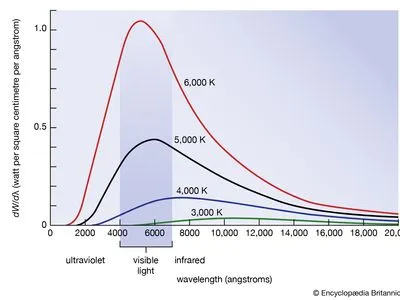
\includegraphics[width=0.6\textwidth]{bb_radiation_distribution.png}
\end{figure}

The emissive power $E_{\lambda}$ is defined as the energy radiated per unit area per unit time per unit wavelength interval. The total energy radiated per unit area per unit time is called the total emissive power $E$. Thus \[
    E_{\lambda} = \frac{\text{Energy radiated per unit area per sec in the range $\lambda$ to $\lambda+d\lambda$}}{\text{Wavelength difference $d\lambda$}}
\]
The total radiation emitted per square meter per second over all wavelengths, i.e the bolometric flux, is represented by \[
    E = \int_{0}^{\infty} E_{\lambda} d\lambda
\]

\subsection{Failure of Classical Physics to Explain Black Body Radiation}

\subsubsection{Wien's Radiation Formula}
\begin{equation}
    E_{\lambda} d\lambda = \frac{C_1}{\lambda^5} \: e^{-C_2/\lambda T} d\lambda
\end{equation}
where $C_1$ and $C_2$ are constants and $T$ is the temperature of the black body. \\~\\

\textbf{Assumptions:} \\
\begin{enumerate}
    \item The radiation inside a hollow enclosure is produced by the oscillation of electrons in the walls of the enclosure.
    \item The frequency of the radiation is proportional to the kinetic energy of the resonator.
    \item The intensity of radiation of a particular wavelength is proportional to the number of resonators having required amount of energy.
    
\end{enumerate}

\textbf{Limitations of the Formula:} \\
The formula explains the experimental results fairly well for short wavelengths, but fails to explain the experimental results for long wavelengths.


\subsubsection{Rayleigh-Jeans Law}
\begin{equation}
    U_{\nu} d\nu = \frac{8\pi\nu^2}{c^3} kT d\nu
\end{equation}
where $U_{\nu}$ is the energy per unit volume per unit frequency range at frequency $\nu$, $k$ is Boltzmann's constant, and $c$ is the speed of light.\\
The formula can also be written in the following form:
\begin{equation}
    U_{\lambda} d\lambda = \frac{8\pi kT}{\lambda^4} d\lambda
\end{equation}

\textbf{Limitations of the Law:} \\
The law explains the experimental results fairly well for long wavelengths, but fails to explain the experimental results for short wavelengths. \\
The law leads to an absurd result that the total energy radiated by a black body is infinite :
\begin{align*}
    U &= \int_{0}^{\infty} {U_{\lambda}} \: d{\lambda} \\
    &= \int_{0}^{\infty} {\frac{8\pi kT}{\lambda^4}} \: d{\lambda} \\
    &= \frac{8\pi kT}{3} \left[ -\frac{1}{3\lambda^3} \right]_{0}^{\infty} \\
    &= \infty
\end{align*}
But experimentally, the total energy radiated by a black body is finite. And $U_{\lambda} d\lambda \to 0$ as $\lambda \to 0$.

\subsection{Planck's Quantum Hypothesis}
Planck assumed that the energy of the oscillators is not continuous, but is quantized. The energy of an oscillator can have only discrete values. The energy of an oscillator is an integral multiple of a basic unit of energy $h\nu$, where $h$ is a constant called Planck's constant and $\nu$ is the frequency of the oscillator. Thus, the energy of an oscillator is given by
\begin{equation}
    E = nh\nu
\end{equation}
As long as the oscillator has energy equal to one of the allowed values given by the relation $E=nh\nu$, it can't emit or absorb energy.

\subsubsection{Planck's Radiation Law}
On the basis of quantum theory, the formula for an average energy of an oscillator can be described as
\begin{equation}
    \boxed{ E = \frac{h\nu}{e^{h\nu/kT}-1} }
\end{equation}

Number of oscillatons or degrees of freedonm per unit volume having frequency between $\nu$ and $\nu+d\nu$ is given by
\begin{equation}
    N(\nu) d\nu = \frac{8\pi\nu^2}{c^3} d\nu
\end{equation}

Assuming that the average value of the energies of the various modes of oscillation in balck body is given by equation (1.3.2), Planck obtained the equation
\begin{equation}
    \boxed{ U_{\nu} d\nu = \frac{8\pi\nu^2}{c^3} \frac{h\nu}{e^{h\nu/kT}-1} d\nu }
\end{equation}
In terms of the wavelength of the radiation, the equation is
\begin{equation}
    \boxed{ U_{\lambda} d\lambda = \frac{8\pi hc}{\lambda^5} \frac{1}{e^{hc/\lambda kT}-1} d\lambda }
\end{equation}

Equations (1.3.4) and (1.3.5) are two forms of Planck's radiation law.

\begin{figure}[htpb]
    \centering
    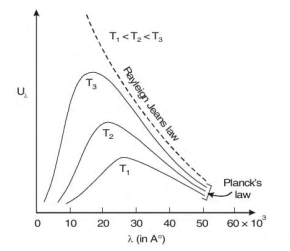
\includegraphics[width=0.55\textwidth]{planck's law.png}
\end{figure}

\subsubsection{Consequences of Planck's Law}
From Planck's law, the Rayleigh-Jeans law, Wien's law, and Stefan's law can be derived as mathematical consequences:

\textbf{(I) Rayleigh-Jeans Law:} \\
\begin{equation}
    U_{\lambda} \: d\lambda = \frac{8\pi hc}{\lambda^5} \frac{1}{hc/\lambda kT} \: d\lambda = \frac{8\pi kT}{\lambda^4} \: d\lambda
\end{equation}

\textbf{(II) Wien's Law:} \\
\begin{equation}
    U_{\lambda} \: d\lambda = \frac{8\pi hc}{\lambda^5} e^{-hc /\lambda kT} \: d\lambda
\end{equation}

\textbf{(III) Wein'd Displacement Law:} \\
\begin{equation}
    U_{\lambda} = \frac{8\pi hc}{\lambda^5} \cdot \frac{1}{e^{hc /\lambda kT} - 1}
\end{equation}

\textbf{(IV) Stefan-Boltzmann Law:} \\
\begin{equation}
    U = \int_{0}^{\infty} U_{\lambda} \: d\lambda = \frac{8\pi^5 k^4}{15c^3 h^3} T^4
\end{equation}
Or,
\begin{equation}
    E = \sigma T^4
\end{equation}
where \[
    \sigma = \frac{2\pi^5 k^4}{15c^2 h^3} = 5.67 \times 10^{-8} \: \text{W m}^{-2} \text{K}^{-4}
\]


\subsection{Photoelectric Effect}
\begin{definition}{Photoelectric Effect}{}
    The phenomenon of emission of electrons from the surface of a metal when light of suitable frequency is incident on it is called photoelectric effect.
\end{definition}

\subsubsection{Experimental Study of Photoelectric Effect}
\begin{figure}[htpb]
    \centering
    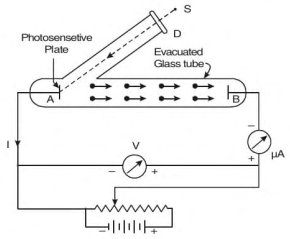
\includegraphics[width=0.5\textwidth]{photoelectric effect.png}
\end{figure}

\begin{enumerate}
    \item The photoelectric current is directly proportional to the intensity of the incident light.
    \item The photoelectric current is directly proportional to the number of photons incident per unit area per unit time.
    \item The photoelectric current is independent of the frequency of the incident light, provided the frequency is greater than a certain minimum value called the threshold frequency.
    \item The maximum kinetic energy of the photoelectrons is independent of the intensity of the incident light.
    \item The maximum kinetic energy of the photoelectrons is directly proportional to the frequency of the incident light.
\end{enumerate}

\textbf{(I) Effect of Frequency of Incident Light on Photoelectric Current:} \\
For a given metal surface, the photoelectric current is zero for light of frequency less than a certain minimum value called the threshold frequency $\nu_0$. The threshold frequency depends on the nature of the metal surface. \\~\\

\begin{figure}[htpb]
    \centering
    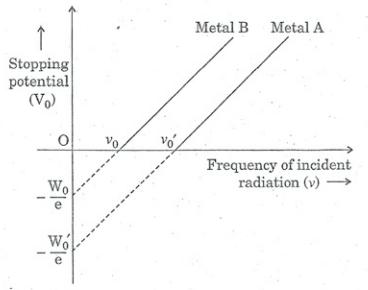
\includegraphics[width=0.3\textwidth]{frequency.png}
    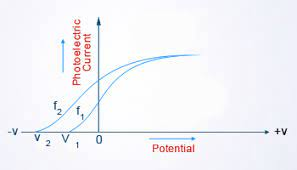
\includegraphics[width=0.4\textwidth]{frequency2.png}
\end{figure}

\textbf{(II) Effect of Intensity of Incident Light on Photoelectric Current:} \\
For a given frequency $\nu > \nu_0$, the photoelectric current is directly proportional to the intensity of the incident light. The number of photoelectrons emitted per second is directly proportional to the intensity of the incident light. \\~\\

\begin{figure}[htpb]
    \centering
    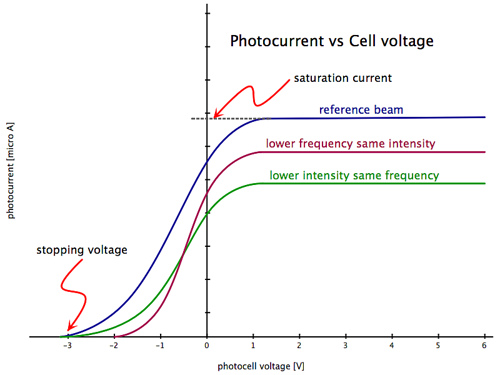
\includegraphics[width=0.5\textwidth]{i vs v.png}
\end{figure}

\textbf{(III) Effect of Potential Difference on Photoelectric Current:} \\
The photoelectric current is zero for a given frequency $\nu > \nu_0$ if the potential difference between the cathode and the anode is less than a certain minimum value called the stopping potential $V_0$. The stopping potential depends on the frequency of the incident light. \[
    \frac{1}{2}m_{e}\nu_{max}^2 = eV_0
\] \\~\\

\textbf{(IV) Effect of Frequency on the Stopping Potential:} \\
For a given metal surface, the stopping potential is directly proportional to the frequency of the incident light. \[
    V_0 \propto \nu
\] \\~\\

\subsubsection{Failure of Classical Physics to Explain Photoelectric Effect}
\textbf{(I) The existence of the threshold frequency:} \\
According to classical physics, the energy of the emitted electrons should depend on the intensity of the incident light and not on its frequency. Thus, the photoelectric effect can't be explained by classical physics. \\~\\

\textbf{(II) The non-dependence of the maximum kinetic energy of the photoelectrons on the intensity of the incident light:} \\
According to classical electromagnetism, oscillating electric vector of the incident radiation should cause an oscillation on the electrons of the metal. If the amplitude of the oscillation is sufficient, the electron is emitted from the surface. Thus, the kinetic energy of the electron must increase with increasing intensity, which doesn't happen in reality. Rather, the maximum kinetic energy of the electron remains the same if the intensity is increased.\\~\\

\textbf{(III) Absence of time lag between the incidence of light and the emission of electrons:} \\
According to wave theory, the electrons should absorb energy continuously from the incident light and should be emitted after a time lag. But in reality, there is no time lag between the incidence of light and the emission of electrons. \\~\\


\subsection{Einstein's Explanation of Photoelectric Effect}
\textbf{Assumptions:} \\
\begin{enumerate}
    \item Light consists of discrete photons or quanta of energy.
    \item The energy of a photon is given by \[
        E = h\nu
    \]
    where $h$ is Planck's constant and $\nu$ is the frequency of the photon.
    \item The energy of a photon is absorbed by a single electron without any time lag. The probability of its absorbing more than one photons at the same time is negligible.
\end{enumerate}

\begin{definition}{Work Function}{}
    The minimum energy required to remove an electron from the surface of a metal is called the work function of the metal. \\
    This energy is taken up by the electron to overcome the attractive forces of the metal atoms.
\end{definition}

\subsubsection{Einstein's Photoelectric Equation}
\begin{equation}
    \boxed{ \frac{1}{2}m_ev_{max}^2 = eV_0 = h\nu - W_0 = h(\nu - \nu_0) }
\end{equation}

\subsubsection{Threshold Frequency}
The threshold frequency $\nu_0$ is the minimum frequency of the incident light for which the photoelectric effect occurs. It is given by \[
    0 = h\nu_0 - W_0
\]
\begin{equation}
    \boxed{ \nu_0 = \frac{W_0}{h} }
\end{equation}

\subsection{Bohr's Quantization of Angular Momentum and Theory of Hydrogen Atom}
\subsubsection{Bohr's Postulates}
\begin{enumerate}
    \item The electron in a hydrogen atom moves in circular orbits around the nucleus.
    \item The electron in a particular orbit has a definite energy and hence a definite radius.
    \item The electron in a particular orbit doesn't radiate energy and hence doesn't lose energy.
    \item The electron can jump from one orbit to another by absorbing or emitting energy.
    \item The angular momentum of the electron in a particular orbit is an integral multiple of $\hbar = h/2\pi$. That is,
        \begin{equation}
            L = mvr = n\hbar = nh/2\pi
        \end{equation}
    where $n = 1, 2, 3, \cdots$
\end{enumerate}
\begin{equation}
    mv^2r = \frac{Ze^2}{4\pi\varepsilon_0}
\end{equation}

\begin{figure}[htpb]
    \centering
    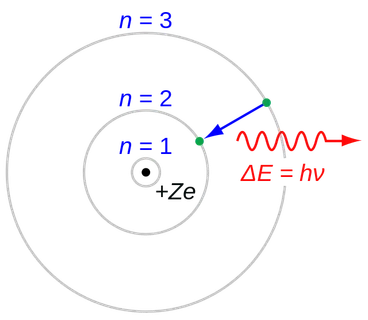
\includegraphics[width=0.3\textwidth]{Bohr's hydrogen.png}
\end{figure}

\subsubsection{Limitations of Bohr's Theory}
\begin{enumerate}
    \item Bohr’s model of an atom failed to explain the Zeeman Effect (effect of magnetic field on the spectra of atoms).
    \item It also failed to explain the Stark effect (effect of electric field on the spectra of atoms).
    \item It violates the Heisenberg Uncertainty Principle.
    \item It could not explain the spectra obtained from larger atoms.
\end{enumerate}


\subsection{Compton Effect}
\begin{definition}{Compton Effect}{}
    The phenomenon of change in wavelength of X-rays when scattered by a material medium is called Compton effect.
\end{definition}

\begin{figure}[htpb]
    \centering
    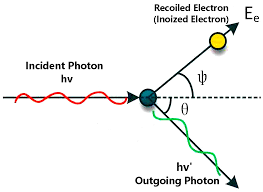
\includegraphics[width=0.4\textwidth]{compton.png}
\end{figure}

\subsubsection{Classical Explanation of Compton Effect}
According to classical physics, the wavelength of the scattered X-rays should be the same as that of the incident X-rays. But in reality, the wavelength of the scattered X-rays is greater than that of the incident X-rays.

\subsubsection{Quantum Theory Explanation of Compton Effect}
Compton explained his experimental results by postulating that incident X-ray beam is an assembly of photons having energy  $E=h\nu$. These photons collide with free electrons in the scattering target. The scattered radiation consists of recoiling photons emerging from the target. The incident photon transfers some of its energy to the free electron, so the scattered photon has less energy than the incident photon. Thus the frequency reduces and wavelength increases.
\begin{equation}
    \boxed{ \Delta \lambda = \lambda' - \lambda = \frac{h}{m_e c} (1 - \cos \theta) }
\end{equation}
where $\theta$ is the angle between the incident and scattered X-rays. \\~\\

%%%%%%%%%%%%%%%%%%%%%%%%%%%%%%%
%  Wave Properties of Matter  %
%%%%%%%%%%%%%%%%%%%%%%%%%%%%%%%

\section{Wave Properties of Matter}
\subsection{Wave Particle Duality}
\begin{definition}{Wave Particle Duality}{}
    The concept that all matter and radiation exhibit both wave-like and particle-like properties is called wave-particle duality.
\end{definition}

\subsection{De Broglie's Hypothesis}
\begin{definition}{De Broglie's Hypothesis}{}
    The hypothesis that every material particle has a wavelength associated with it is called De Broglie's hypothesis.
\end{definition}

According to Planck-Einstein equation, the energy of a photon is given by
\begin{equation}
    E = h\nu
\end{equation}
According to theory of relativity,
\begin{equation}
    E^2 = (pc)^2 + (m_0c^2)^2
\end{equation}
where $p$ is the momentum of the photon, $m_0$ is the rest mass of the photon, and $c$ is the speed of light. \\
Since the photon has no rest mass, equation (2.2.2) reduces to \[
    E^2 = p^2c^2
\]
\begin{equation}
    p = \frac{E}{c}
\end{equation}
Substituting equation (2.2.1) in equation (2.2.3), we get \[
    p = \frac{h\nu}{\nu\lambda} = \frac{h}{\lambda}
\]
\begin{equation}
    \boxed{ \lambda = \frac{h}{p} }
\end{equation}
This equation represents the wave-particle relation for photons. Here, $\lambda$ is the wavelength associated with photons of momentum $p$. \\
Thus, the relativistic expression for the momentum of a photon can be given by
\begin{equation}
    \boxed{ p = \frac{m_0v}{\sqrt{1-\frac{v^2}{c^2}}} }
\end{equation}
According to De Broglie's hypothesis, every material particle has a wavelength associated with it. Hence, we can write 
\begin{equation}
    \boxed{ \lambda = \frac{h}{p} = \frac{h}{mv} }
\end{equation}
where $m$ is the mass of the particle and $v$ is its velocity. \\
If $E_K$ is the kinetic energy of the particle, then \[
    E_K = \frac{1}{2}mv^2 = \frac{p^2}{2m}
\]
Hence, the momentum of the particle is given by
\begin{equation}
    \boxed{ p = \sqrt{2mE_K} }
\end{equation}
Therefore, the wavelength associated with the particle is given by
\begin{equation}
    \boxed{ \lambda = \frac{h}{\sqrt{2mE_K}} }
\end{equation}

\subsubsection{Rest Mass of a Photon}
The relativistic expression for the momentum of a photon is given by \[
    p = \frac{m_0v}{\sqrt{1-\frac{v^2}{c^2}}}
\]
From quantum theory of radiation, \[
    p = \frac{h}{\lambda}
\]
Therefore, \[
    \frac{h}{\lambda} = \frac{m_0v}{\sqrt{1-\frac{v^2}{c^2}}}
\]
Hence, the rest mass of a proton is \[
    m_0 = \frac{h}{v\lambda} \sqrt{1-\frac{v^2}{c^2}} = \frac{h}{c\lambda} \sqrt{1 - \frac{c^2}{c^2}} = 0
\]


%%%%%%%%%%%%%%%%%%%%%%%%%%%%%%%%%%%%%%%%
%  Heisenberg's Uncertainty Principle  %
%%%%%%%%%%%%%%%%%%%%%%%%%%%%%%%%%%%%%%%%

\section{Heisenberg's Uncertainty Principle}

\begin{definition}{Heisenberg's Uncertainty Principle}{}
    The principle states that for a particle of atomic magnitude, in motion, it is impossible to determine both the position and the momentum simultaneously with perfect accuracy.
\end{definition}

\subsection{Uncertainty in Position and Momentum}
Quantitative statement of the principle is given by
\begin{equation}
    \boxed{ \Delta x \Delta p \geq \frac{\hbar}{2} }
\end{equation}
where $\Delta x$ is the uncertainty in the position of the particle and $\Delta p$ is the uncertainty in the momentum of the particle. And $\displaystyle \hbar = \frac{h}{2\pi}$ \\

\subsection{Uncertainty in Energy and Time}
The uncertainty principle can also be stated in terms of energy and time as
\begin{equation}
    \boxed{ \Delta E \Delta t \geq \frac{\hbar}{2} }
\end{equation}

\subsection{Uncertainty in Angular Position and Angular Momentum}
The uncertainty principle can also be stated in terms of angular position and angular momentum as
\begin{equation}
    \boxed{ \Delta \theta \Delta L \geq \frac{\hbar}{2} }
\end{equation}

\subsection{Application: Absence of Electrons in the Nucleus}
The radius of the nucleus is of the order of $10^{-15}$ m. If an electron is present in the nucleus, then the uncertainty in its position is of the order of $10^{-15}$ m. Hence, the uncertainty in its momentum is given by \[
    \Delta p \geq \frac{\hbar}{2\Delta x} = \frac{h}{4\pi\Delta x} = \frac{6.63 \times 10^{-34}}{4 \times 3.14 \times 10^{-15}} = 5.3 \times 10^{-20} \: \si{kg m s}^{-1}
\]
Thus, the momentum of the electron must be \textit{at least} equal to the above value. As we know, $p = m_e v$. Thus, for the electron to be inside the nucleus, the velocity would be \[
    v = \frac{p}{m_e} = \frac{5.3 \times 10^{-20}}{9.1 \times 10^{-31}} = 5.8 \times 10^{10} \: \si{m s}^{-1}
\]
Here, $v > c$, which is not possible. Hence, we can conclude that, an electron can't exist inside the nucleus of an atom.



%%%%%%%%%%%%%%%%%%%%%%%%%%%%%%%%%
%  Schrodinger's Wave Equation  %
%%%%%%%%%%%%%%%%%%%%%%%%%%%%%%%%%

\section{Schrodinger's Wave Equation}
\subsection{Schrodinger's One-Dimensional Time-Dependent Wave Equation}
\subsubsection{Wave Function for a Free Particle}
Let a particle of mass $m$ be in motion in the positive $x$ direction with velocity $v$, accurately known momentum $p_x$ and total energy $E$. The position of the particle would be completely undetermined. The wave associated with such a particle should be a plane continuous simple harmonic wave travelling in the positive $x$ direction.\\~\\
In wave mechanics, the wave function $\psi$ is a function of $x$ and $t$. Thus, the wave function of the particle is given by
\begin{equation}
    \boxed{ \psi(x, t) = A e^{i(kx - \omega t)} }
\end{equation}
where $A$ is the amplitude of the wave, $k$ is the wave number, and $\omega$ is the angular frequency of the wave. \\~\\

The momentum of the particle is given by
\begin{align*}
    p_x &= \frac{h}{\lambda} = \frac{h}{2\pi}\frac{2\pi}{\lambda} \\
    &= \hbar k \\
    &= \hbar \frac{2\pi\nu}{v}
\end{align*}
\begin{equation}
    \frac{\omega}{v} = \frac{p_x}{\hbar}
\end{equation}
Energy of the particle is given by
\begin{align*}
    E &= h\nu = \frac{h}{2\pi}2\pi\nu \\
    &= \hbar \omega
\end{align*}
\begin{equation}
    \omega = \frac{E}{\hbar}
\end{equation}

Substituting the expressions in equation (4.1.1), we get
\begin{equation}
    \boxed{ \psi(x, t) = A e^{\frac{i}{\hbar}\left( p_{x}x - Et \right)} }
\end{equation}

\subsubsection{One-Dimensional Time-Dependent Wave Equation}
If the speed of the particle is small compared to that of light, the total energy is
\begin{equation}
    E = E_K + E_P = \frac{p_{x}^2}{2m} + V
\end{equation}
If the motion of the particle is due to the action of a force $F(x)$ which is a function of $x$, then $V$ will be a function only of $x$. Multiplying both sides of equation (4.1.5) by the wave function $\psi(x,t)$, we get
\begin{equation}
    \frac{p_x^2 \psi}{2m} + V\psi = E\psi
\end{equation}

Differentiating equation (4.1.4) with respect to $x$, we get
\begin{align*}
    \pdv{\psi}{x} &= A \left( \frac{i}{\hbar} \right)p_x e^{i/\hbar (p_x x - Et)} \\
    &= \left( \frac{i}{\hbar} \right) p_x A e^{i/\hbar (p_x x - Et)}
\end{align*}
\begin{equation}
    \pdv{\psi}{x} = \left( \frac{i}{\hbar} \right) p_x \psi
\end{equation}
\begin{align*}
    \pdv[2]{\psi}{x} &= \left( \frac{i}{\hbar} \right) p_x \pdv{\psi}{x} \\
    &= \left( \frac{i}{\hbar} \right) p_x \left( \frac{i}{\hbar} \right) p_x \psi \\
    &= -\frac{1}{\hbar^2} p_x^2 \psi
\end{align*}
Thus we have
\begin{equation}
    p_{x}^2 \psi = -\hbar^2 \pdv[2]{\psi}{x}
\end{equation}\\~\\

Now, differentiating equation (4.1.4) with respect to $t$, we get
\begin{align*}
    \pdv{\psi}{t} &= A \left( \frac{i}{\hbar} \right) E e^{i/\hbar (p_x x - Et)} \\
    &= \left( \frac{i}{\hbar} \right) (-E) A e^{i/\hbar (p_x x - Et)} \\
    &= -\frac{i}{\hbar} E \psi
\end{align*}
\begin{equation}
    E\psi = -\frac{\hbar}{i} \pdv{\psi}{t}
\end{equation}

Substituting these expressions for $p_{x}^2\psi$ and $E\psi$ in equation (4.1.6), we get
\begin{equation}
    \boxed{ -\frac{\hbar^2}{2m} \pdv[2]{\psi}{x} + V\psi = -\frac{\hbar}{i} \pdv{\psi}{t} }
\end{equation}
This is the one-dimensional time-dependent wave equation. \\~\\

In three dimensions, the wave equation is given by
\begin{equation}
    \boxed{ \left[ -\frac{\hbar^2}{2m} \nabla^2 + V \right] \psi = -\frac{\hbar}{i} \pdv{\psi}{t} }
\end{equation}
where $\displaystyle \nabla^2 = \left( \pdv[2]{\psi}{x} + \pdv[2]{\psi}{y} + \pdv[2]{\psi}{z} \right)$ is the Laplacian operator.


\subsection{Schrodinger's One-Dimensional Time-Independent Wave Equation}
The one-dimensional time-dependent wave equation is given by
\begin{equation}
    -\frac{\hbar^2}{2m} \pdv[2]{\psi}{x} + V\psi = -\frac{\hbar}{i} \pdv{\psi}{t} 
\end{equation}
Equation (4.2.1) is a partial differential equation in two variables $(x,t)$. The equation is separable into the time-independent part and time-dependent part, if the potential energy $V$ is a function of $x$ only, and the total energy $E$ is constant.\\
Let $u(x)$ and $f(t)$ be the time-independent and time-dependent parts respectively. Then
\begin{equation}
    \psi(x,t) = u(x)f(t)
\end{equation}

Substituting this in equation (4.2.1), we get
\begin{equation}
    -\frac{\hbar^2}{2m} f \dv[2]{u}{x} + Vuf = -\frac{\hbar}{i} u \dv{f}{t}
\end{equation}

Dividing both sides by $uf$, we get
\begin{equation}
    -\frac{\hbar^2}{2m} \frac{1}{u} \dv[2]{u}{x} + V = -\frac{\hbar}{i} \frac{1}{f} \dv{f}{t}
\end{equation}

The RHS of this equation is a function of only time $t$, and the LHS is a function of only $x$. \\
Now, we can make use of equation (4.1.9) to write
\begin{equation}
    -\frac{\hbar}{i} \frac{1}{f} \dv{f}{t} = E
\end{equation}
This is the time-dependent part of Schrodinger's equation.\\~\\
Now, from equations (4.2.3) and (4.2.4), we get
\begin{equation}
    -\frac{\hbar^2}{2m} \frac{1}{u} \dv[2]{u}{x} + V = E
\end{equation}
Multiphying both sides by $u$, and rearranging, we get
\begin{equation}
    \boxed{ \dv[2]{u}{x} + \frac{2m}{\hbar^2} (E-V)u = 0 }
\end{equation}
This is the one-dimentional time-dependent Schrodinger's equation.\\~\\
In three dimensions, the time-independent Schrodinger's equation is given by
\begin{equation}
    \boxed{ \nabla^2 u + \frac{2m}{\hbar^2} (E-V)u = 0 }
\end{equation}

\subsection{The Infinite Square Well Potential}
Consider a particle of mass $m$ moving inside a box along the $x$ direction. The particle is bouncing back and forth between the walls of the box. The box has insurmountable potential barriers at $x=0$ and $x=L$.\\
The potential energy $V$ of the particle is infinite on both sides of the box, and $V=0$ between $x=0$ and $x=L$.\\~\\

Within the box, the Schrodinger's equation is given by
\begin{equation}
    \dv[2]{\psi}{x} + \frac{2m}{\hbar^2} E\psi = 0
\end{equation}

\begin{figure}[htpb]
    \centering
    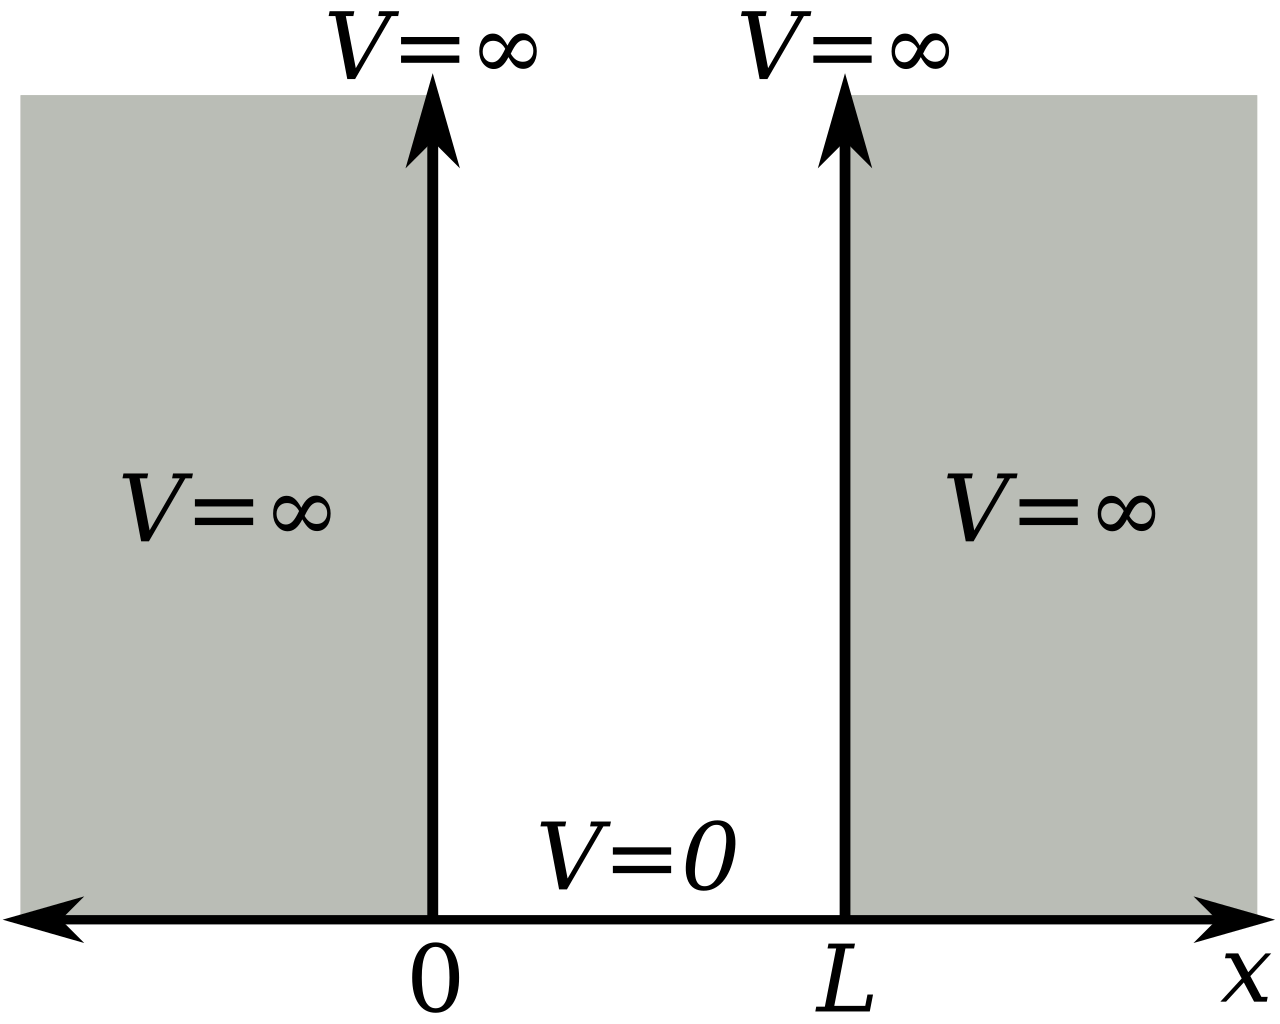
\includegraphics[width=0.3\textwidth]{potential well.png}
\end{figure}

The general solution of this equation is
\begin{equation}
    \psi = A \sin{\frac{\sqrt{2mE}}{\hbar}x} + B \cos{\frac{\sqrt{2mE}}{\hbar}x}
\end{equation}
where $A$ and $B$ are constants to be evaluated.\\~\\

The boundary conditions are
\begin{enumerate}[(i)]
    \item $\psi=0$ at $x=0$. Hence, $B=0$.
    \item $\psi=0$ at $x=L$. Hence, $\displaystyle \sin{\frac{\sqrt{2mE}}{\hbar}L} = 0$.\\
\end{enumerate}
Thus
\begin{equation}
    \frac{\sqrt{2mE}}{\hbar}L = n\pi \qquad n=1,2,3,\cdots
\end{equation}

Thus, the energy of the particle is given by
\begin{equation}
    \boxed{ E_n = \frac{n^2\pi^2\hbar^2}{2mL^2} }
\end{equation}

\subsubsection{Wave Function}
The wave function of the particle inside the box is, where energies are $E_n$ is given by
\begin{equation}
    \psi_n = A \sin{\frac{\sqrt{2mE_n}}{\hbar}x}
\end{equation}
Substituting the value of $E_n$ in equation (4.3.4), we get
\begin{equation}
    \boxed{ \psi_n = A \sin{\frac{n\pi x}{L}} }
\end{equation}

\subsubsection{Evaluation of $A$ and Normalization of the Wave Function}
It is certain that the particle is somwhere inside the box. Hence, for a normalised wave function
\begin{minipage}{0.45\textwidth}
    \begin{align*}
        \int_{0}^{L} {\psi\cdot\psi^{*}} \: d{x} &= 1 \\
        A^2 \int_{0}^{L} {\sin^2{\left( \frac{n\pi x}{L} \right)}} \: d{x} &= 1 \\
        A^2 \int_{0}^{L} {\left( \frac{1 - \cos{\left( \frac{2n\pi x}{L} \right)}}{2} \right)} \: d{x} &= 1 \\
        A^2 \frac{L}{2} &= 1 \\
        A &= \sqrt{\frac{2}{L}}
    \end{align*}

\end{minipage}
\begin{minipage}{0.6\textwidth}
    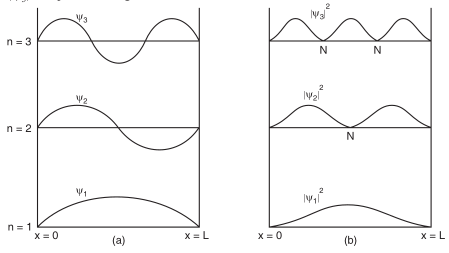
\includegraphics[width=0.8\textwidth]{potential well2.png}
\end{minipage}\\~\\

The normalised wave function thus is given by
\begin{equation}
    \boxed{ \psi_n = \sqrt{\frac{2}{L}} \sin{\frac{n\pi x}{L}} } \qquad n=1,2,3,\cdots
\end{equation}

\subsection{Potential Step}
The potential function of a potential step is defined by
\begin{equation}
    V(x) = \begin{cases}
        0 & \text{if } x < 0 \\
        V_0 & \text{if } x > 0
    \end{cases}
\end{equation}

The time-independent Schrodinger's equation is given by
\begin{equation}
    \dv[2]{\psi}{x} + \frac{2m}{\hbar^2} (E-V)\psi = 0
\end{equation}
For region (I), $V=0$. Hence, the equation is given by
\begin{equation}
    \dv[2]{\psi}{x} + \frac{2mE}{\hbar^2} \psi = 0
\end{equation}

\begin{figure}[htpb]
    \centering
    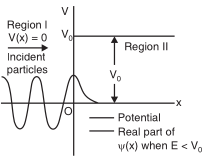
\includegraphics[width=0.3\textwidth]{potential step.png}
\end{figure}

The solution of equation (4.4.3) is
\begin{equation}
    \psi_1 = A e^{ip_1x/\hbar} + B e^{-ip_1x/\hbar}
\end{equation}
where $A$ and $B$ are constants. And \[
    p_1 = \sqrt{2mE}
\]
Some particles may be reflected by the potential barrier and some transmitted. The first and second terms represent the \textit{incident} and \textit{reflected} particles. \\~\\

The Schrodinger's wave equation for region (II) is given by
\begin{equation}
    \dv[2]{\psi}{x} + \frac{2m}{\hbar^2} (E-V_0)\psi = 0
\end{equation}
The solution of equation (4.4.5) is
\begin{equation}
    \psi_2 = C e^{ip_2x/\hbar} + D e^{-ip_2x/\hbar}
\end{equation}
where $C$ and $D$ are constants. And \[
    p_2 = \sqrt{2m(E-V_0)}
\]
In equation (4.4.6), the first term represents the \textit{transmitted wave}, and the second term represents a wave coming from $+\infty$ in the negative direction. For $x>0$, no particle can flow to the left and $D$ must be zero. Therefore equation (4.4.6) becomes
\begin{equation}
    \psi_2 = C e^{ip_2x/\hbar}
\end{equation}
The continuity of $\psi$ implies that $\psi_1=\psi_2$ at $x=0$. Hence,
\begin{equation}
    A + B = C
\end{equation}
Also, the continuity of $\psi$ implies that $\displaystyle \dv{\psi_1}{x} = \dv{\psi_2}{x}$ at $x=0$.\\
Therefore,
\begin{equation}
    p_1(A-B) = p_2C
\end{equation}
Solving equations (4.4.8) and (4.4.9), we get
\begin{align}
    B &= \frac{p_1-p_2}{p_1+p_2} A \\
    C &= \frac{2p_1}{p_1+p_2} A
\end{align} \\~\\

Now, two cases may arise:
\begin{enumerate}[(i)]
    \item $E > V_0$ :\\
        $\psi$ is a travelling wave, but of differing wave number from the incident wave.
    \item $E < V_0$ :\\
        $\alpha$ is imaginary. Therefore $\psi$ is a decaying exponential. \[
            \psi = Ce^{i\alpha x} = Ce^{-\frac{\sqrt{2m(V_0-E)}}{\hbar}x}
        \]
\end{enumerate}

\end{document}
